\section{Zielsetzung}
In diesem Versuch wird der Effekt der Faraday Rotation verwendet um die
effektive Masse der Leitungselektronen in n-dotierten Galliumarsenid zu messen.

\section{Theorie}
In diesem Versuch scheint eine polarisierte elektromagnetische Welle durch
einen Halbleiter. Dieser Halbleiter wird einem Magnetfeld ausgesetzt was zu
einer Verdrehung der Polarisationsachse führt. Diese Begriffe werden im
folgenden definiert

\subsection{Halbleiter \cite[][Kap. 14]{book:expi3}}
Elektronen in Festkörpern haben anstelle von diskret definierten Zuständen
aufenthaltswahrscheinlichkeiten in der Form von Bändern. Leitende Festkörper
zeichnen sich durch Elektronen im ungebundenen Zustand aus. Isolatoren wiederum
haben eine große Bandlücke zwischen den Gebundenen Elektronen und dem ersten
freien Leitungsband. Diese Bandlücke ist bei Halbleitern in der Größenordnung
von etwa $\qty{1}{\eV}$. Die Bandstruktur von Halbleitern ist auch eine Funktion
des Impuls der Elektronen bzw. des Wellenvektors $\vec{k}$

\subsection{Effektive Masse}

Vielleicht braucht man ja diese Formeln:
\begin{align}
	E                 & = E_L + \frac{\hbar k²}{2 m_e}                 \\
	\frac{d v_g}{d t} & = \frac{1}{\hbar^2}\frac{d^2 E}{d^2 k} \vec{F} \\
	m^*               & = \hbar^2 \cdot \frac{d²E}{d k_i d k_j^{-1}}
	E_e(\vec{k})      & = \frac{\hbar²}{3m^*_e}
\end{align}

\subsection{Fehlerrechnung}
Für die Fehlerrechnung werden alle \textbf{Mittelwerte} von $N$ Messungen
folgendermaßen berechnet:

\begin{equation}
	\overline{x} = \frac{1}{N} \cdot \sum_{i=1}^N x_i
	\label{eqn:Mittelwert}
\end{equation}

und alle \textbf{Standardabweichungen zum Mittelwert} mit:

\begin{equation}
	\increment\overline{x} = \sqrt{\frac{1}{N\cdot(N-1)}\cdot\sum_{i=1}^N (x_i-\overline{x})^2}
	\label{eqn:St_Mittelwert}
\end{equation}

Der Fehler für zusammenhängende Messwerte wird dann mit der \textbf{Gaußschen
	Fehlerfortpflanzung} berechnet:

\begin{equation}
	\increment{f} = \sqrt{ \sum_{i = 1}^{N}  \biggl(\frac{\partial{f}}{\partial{x_i}}\biggr)^2\cdot(\increment{x_i})^2}
	\label{eqn:Gauss}
\end{equation}

Die Fehlerfortpflanzung wird mit Uncertainties in Python \cite{uncertainties}
ermittelt.

%---------------------------------------------------------------------------------------------------------------------------------------------------------------%

\section{Durchführung\cite{man}}% TODO Zahlen überprüfen
Zwei Spulen werden hintereinander mit einem konstanten Strom von
$\qty{10}{\ampere}$ versorgt. Eine Hallsonde wird durch die Spule geschoben um
die Magnetfeldverteilung zu messen. Die Proben werden im Versuch in der
Mitte der Spule eingespannt wo das Magnetfeld am stärksten ist.

Der Versuch wird wie in Abbildung \ref{fig:aufbau} aufgebaut. Weißes licht wird
in einem einstellbaren Polarisator polarisiert und scheint durch die Spule. Im
Zentrum der Spule wird bei dem höchsten Magnetfeld eine Probe mit einer % Hier die Sorten der Proben einfügen
bekannten Elektronenlochdichte eingespannt. Das Licht fällt danach auf ein
Glen-Thomson Prisma. Es spaltet das Licht in zwei Teile mit zueinander
senkrechter linearer Polarisation. Die beiden Photowiderstände geben ihr Signal
weiter an einen Differenzverstärker. Dessen Signalspannung ist proportional zu
dem Intensitätsunterschied zwischen den beiden Polarisationsachsen. Wenn die Signalspannung des 
Differenzverstärkers null (bzw. minimal) wird, ist die Polarisation genau diagonal zu dem Prisma.
Um das Rauschen der Photowiderstände von dem Lichtsignal zu unterscheiden wird zusätzlich der  

Der Faraday Effekt rotiert die Polarisationsebene des Lichtes um den Winkel $\theta$.
Das mit einem Goniometer einstellbare Glen-Thomson-Prisma wird auf den Winkel gedreht, bei dem
die differenzspannung minimal ist. 

\begin{figure}
	\centering
	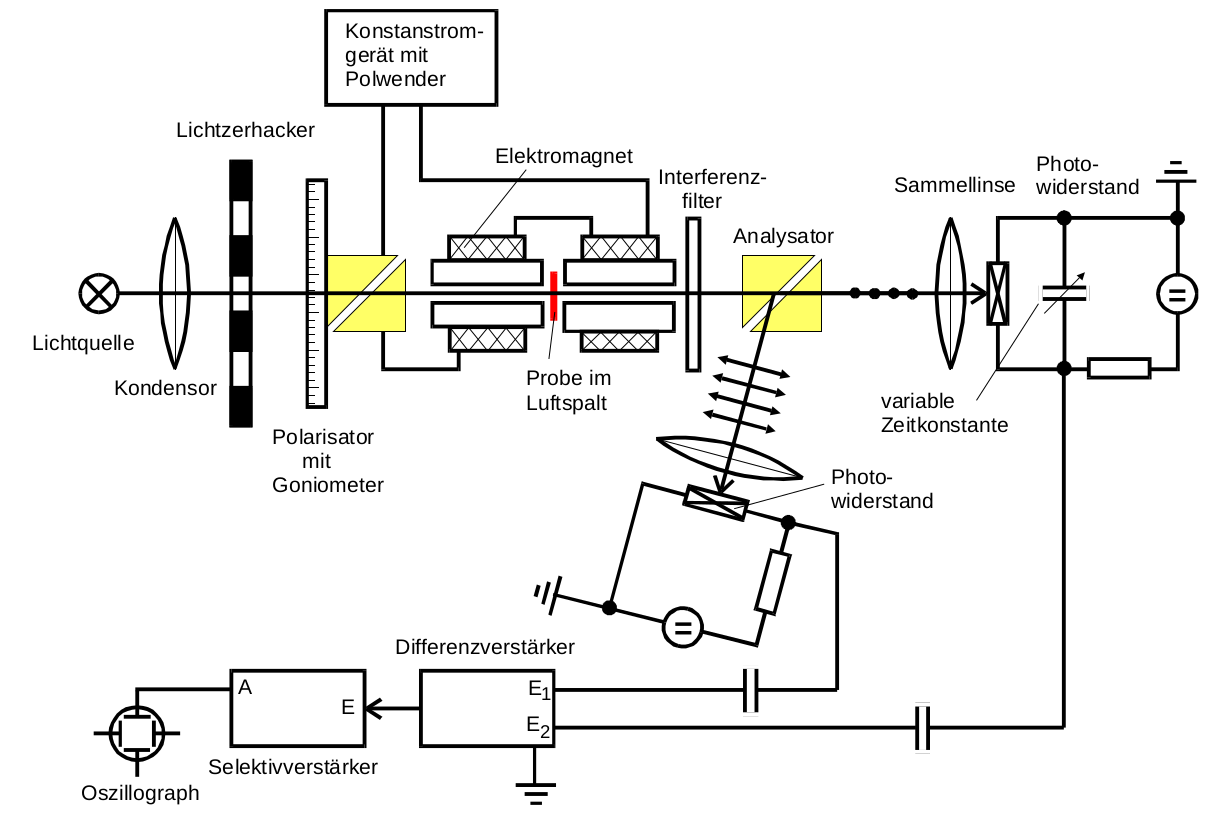
\includegraphics[width=0.8\textwidth]{./Bilder/aufbau.png}
	\caption{Der Versuchsaufbau \cite{man}}\label{fig:aufbau}
\end{figure}

